\documentclass{report}

\pdfpagewidth 8.5in
\pdfpageheight 11in
% \setlength\topmargin{0in}
% \setlength\headheight{0in}
% \setlength\headsep{0in}
% \setlength\textheight{7.7in}
\setlength\textwidth{6.5in}
\setlength\oddsidemargin{0in}
\setlength\evensidemargin{0in}
% \setlength\parindent{0.25in}
% \setlength\parskip{0.25in} 

\pagestyle{headings}
\usepackage{url}
\usepackage[dvips]{graphicx}

\author{Geoff Lawler \url{<geoff.lawler@cobham.com>}}
\title{{\bf Watcher Improvements Project}\\Wrap-up Report FY08}
% \subtitle{The Search for Spock}

\begin{document}
\maketitle

\renewcommand*\thesection{\arabic{section}}

\section{Introduction}

``The Watcher'' is a MANET visualization tool that allows researchers to visualize the locations and states of nodes in an emulated MANET environment. The watcher was originally written 
as a quick and dirty debugging tool used to verify that the MANET emulation tools were working properly. By being able to visualize the locations of the nodes, it was easy to 
tell if the mobility scenario was working and the node connectivty appeared correct. Quickly after this the ability to display text labels on nodes and edges of the connectivity 
graph was added to enable researchers to debug the inner workings of the MANET security tools they were developing on their MANET emulation test beds. The ability to display labels
allowed the state of any node to be seen at a glance. The watcher was found to be a useful tool and was used by a fair number of reasearchers in the community. 

In the summer of 2007, ARL approached SPARTA with the of funding a small project not only to enhance the watcher in order to make it a better tool for research, but enhance 
its graphics for use in demos. The contract and statement of work was finalized and a kickoff meeting was had in August of 2008. Now in August of 2009 the contract is ending and 
this report hopes to briefly summarize the work done, findings, and possible future directions for watcher improvements. 

Figure \ref{fig:oldWatcher} shows the watcher tool at the start of the improvements project. Figures \ref{fig:legWatcherGUI} and \ref{fig:watcherWithBackground}
show the watcher towards the end of the improvments contract. Note that the GUI is now in a window and contains user interface elements such as buttons, menus, and playback
mechanism, a background image,  etc. Because of updates to the watcher architecture, it is now possible to have multiple distinct GUIs displaying the same (live or recorded) data. So in addition to improving
work on the original watcher GUI, some work was done exploring more advanced graphical development environments and writing new watcher GUIs from scratch. (This is why the original
GUI is sometimes refered to as the ``legacy watcher''.) A proof of concept using an advanced game-engine can be seen in figure \ref{fig:ogreWatcherGUI}. 

\begin{figure}[htb]
\centering
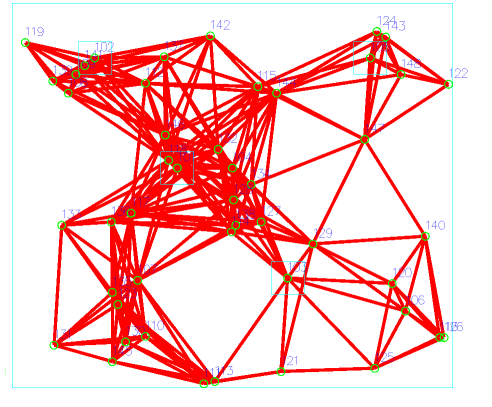
\includegraphics[width=0.5\textwidth]{oldWatcher.eps}
\caption{Watcher at start of project}
\label{fig:oldWatcher}
\end{figure}

\begin{figure}[htb]
\centering
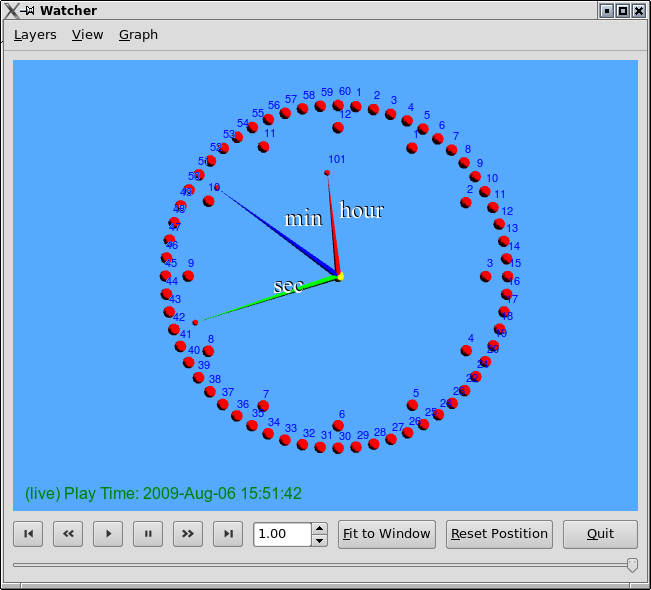
\includegraphics[width=0.5\textwidth]{legWatcherGUI.eps}
\caption{``Legacy Watcher'' at end of project. Note user interface widgets.}
\label{fig:legWatcherGUI}
\end{figure}

Below are three sections that give an overview of the work done in the last year on the watcher improvements project. First
is the work accomplished - what was done and why. This is followed by a section on lessons learned from the work done. What is now known 
that was not known then? What would be done differently if given the chance? The final section gives a recommendation on future directions
for the project. Where the watcher system may go and how it will get there. 

\section{Work Performed}

\subsection{Watcher Improvements}
The main watcher GUI had many updates and fixes applied in the first half on the contract. This portion of the time was focused on updating the GUI to 
support usability and display features for the Army Science Conference in December. Thus the focus was on modifying the existing code base - fixing bugs, 
and adding features requested by ARL. The last six months of the contract focused much more on the new architecture, full ``TiVO'' mode, and removing 
the reliance on the hierarchy daemons as a transport mechanism. The second half on the contract saw a large amount of code written, new GUIs developed, and 
a near complete rewrite of the existing watcher GUI. 

Here is a list of updates and bug fixes applied in the first half of the contract.

\begin{itemize}
\item Wrapped the OpenGL window in a Qt window, giving us modern GUI widgets. 
\item Use mouse to control movement in the main watcher window.
\item More modular logging. Good for debugging and general system performance.
\item Graphical primitives in watcher window are 3d. Can toggle between 3d and 2d via a menu.
\item Added ability to load a background image into main watcher GUI window and place it as needed via the mouse.
\item Watcher GUI saves state to human readable configuration file on exit. This file is also read on start and watcher honors the 
settings found there. File can be edited to modify watcher GUI behavior.
\item Test nodes can control how they are represented in the GUI (shape, size, color, flashing, spinning, blinking, etc). These representations
are saved in the watcher configuration file.
\item Can use the mouse to select a node in the GUI.

\item Added 2d scrolling graph to watcher GUI. Test nodes send periodic data to the watcher. The watcher saves this information and when 
a user clicks on a node, the data stored by the watcher is displayed. Multiple test node's data can be displayed at once and the graph
works in real time, as new data comes in, the old data is scrolled off the end of the graph dialog. Multiple types of period data 
supported. (Although the types are hard-coded. In the second half of the project, these were made dynamic.) See figure \ref{fig:watcherBandwidthGraphDialog} 
for an example snapshot.

\begin{figure}[htb]
\centering
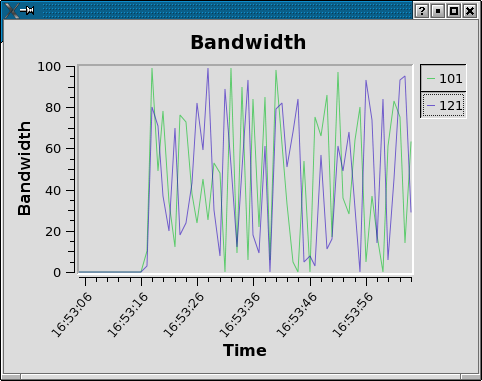
\includegraphics[width=0.4\textwidth]{watcherBandwidthGraphDialog.eps}
\caption{Example of 2d scrolling graph in ``legacy watcher''}
\label{fig:watcherBandwidthGraphDialog}
\end{figure}

\item Background color of the GUI can be changes at run-time. New color is saved in watcher configuration file.
\end{itemize}

\begin{figure}[htb]
\centering
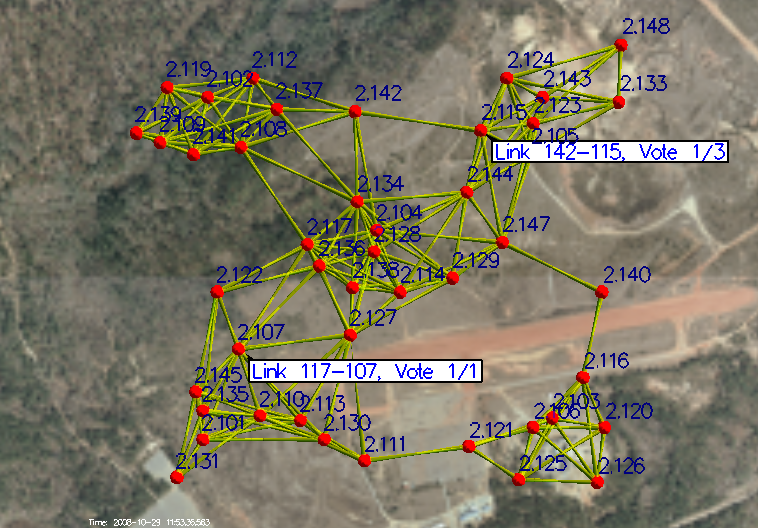
\includegraphics[width=0.5\textwidth]{watcherWithBackground.eps}
\caption{``Legacy Watcher'' showing background and 3D primitives}
\label{fig:watcherWithBackground}
\end{figure}

The second half of the contract focused on a new watcher architecture, designed to support full ``TiVO'' mode, fully dynamic system, removing reliance
on hieraxhy daemons as a transport mechanism. Below is a list of highlights from this half of the project.

\begin{itemize}
\item Wrote new watcher messaging system including message parsing, protocols, and message formats from scratch. 
\item Split message handling, message playback, and message caching from graphical representation. Architecture now
supports a single daemon and multiple different GUIs. 
\item Watcher daemon now uses database to store messages for playback instead of binary blob file format. This allows
flexibility and the ability of third-party applications to process watcher data. 
\item Rewrote all network code, creating the watcher daemon and removing GUI reliance on hierarchy. Network functionality is now
much more scalable. 
\item Wrote proof of concept watcher GUI based on the Object-Oriented Graphical Rendering Engine (OGRE). See figure \ref{fig:ogreWatcherGUI} for a 
screen shot. (Note that the robots can be easily swapped out for tanks or other more military-oriented figures.) 

\begin{figure}[htb]
\centering
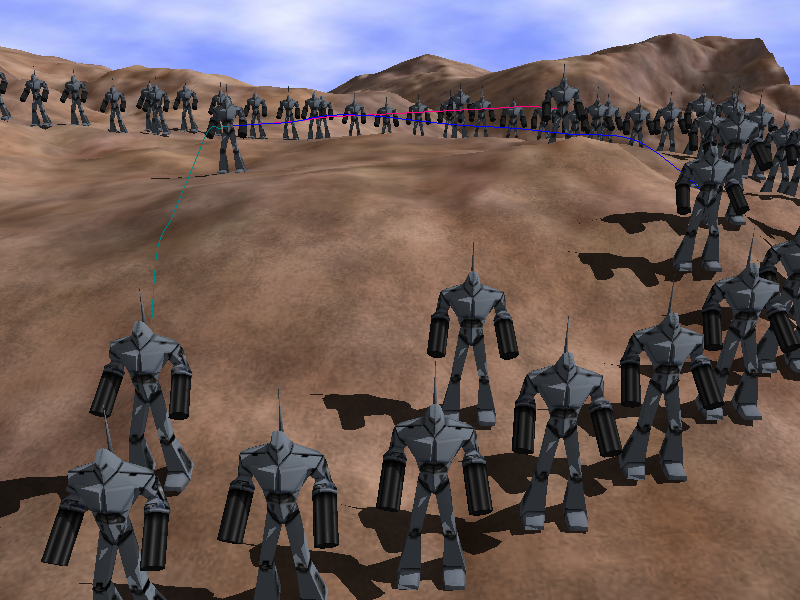
\includegraphics[width=0.8\textwidth]{ogreWatcherGUI.eps}
\caption{First cut at game engine-based watcher GUI. The watcher of the future?}
\label{fig:ogreWatcherGUI}
\end{figure}

\item The watcher GUI now supports fully dynamic layers and graph data. No layer or graph data is hard-coded in the watcher system, all 
the layer and graph data is fed directly from test nodes and handled in the GUI in a simple and systematic way.
\item Investigated use of Google Earth for a watcher system GUI. It appears feasible. 
\item Investigated The Delta-3D game engine as the basis of a new watcher GUI. Wrote proof of concept application. 
\item Wrote test node daemon that runs on test nodes and converts old hierarchy-based watcher messages into new message format. 
This means that old watcher-aware daemons do not have to be updated to support the new transport mechanism.
\item Wrote new watcher GPS daemon that supports the new GPS daemon that {\it emane} uses (gpsd). 
\end{itemize}

\subsection{New Architecture}

The watcher architecture was redesigned and abstract to promote flexibility and extensibility. Divorcing the record 
capability from the display mechanism allowed us to easily add full "TiVO" capability and the ability to have multiple 
GUIs with independent views into the same data set. One researcher can view a test run which focuses on a single node of region, 
pausing and fast-forwarding a single section of the playing field while another researcher can view it all or jump from 
location to location, viewing multiple different layers of the data set. See figure \ref{fig:watcherArch} for a diagram 
of the new architecture.

\begin{figure}[htb]
\centering
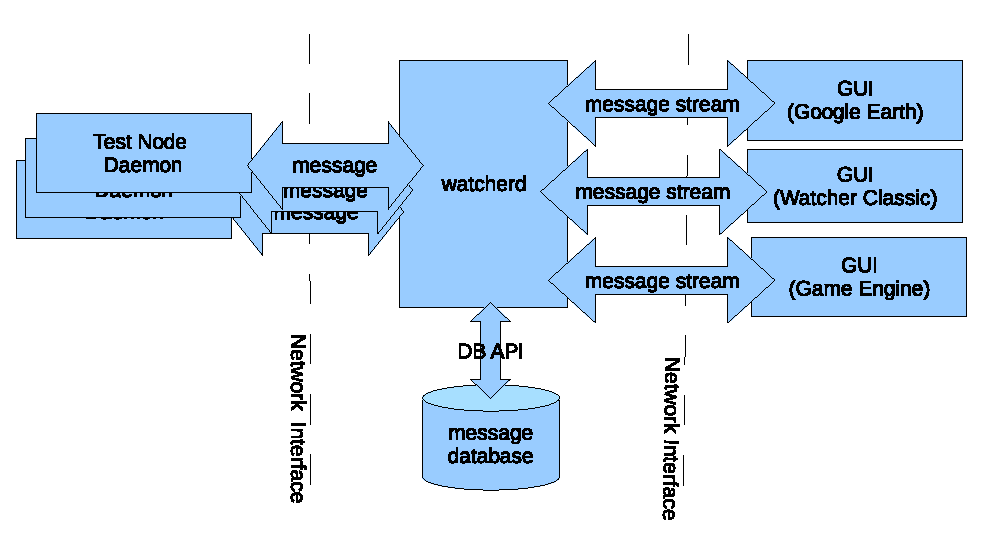
\includegraphics[width=0.8\textwidth]{watcherArch.eps}
\caption{New watcher system architecture}
\label{fig:watcherArch}
\end{figure}

Abstracting the layer concept allows the researcher to add layers dynamically at run-time. For example, 
if a researcher notices a problem with bandwidth usage, he or she can easily write a new test node daemon that 
adds a new ``bandwidth'' layer to the data set. This new layer shows up in the GUI and can be toggled as needed. 
Compare this to the old watcher which had a fixed, hard-coded set of layers regardless of the components of the test
of the researches needs. The old watcher always had a ``wormhole attacks'' layer even if the test did not 
contain the wormhole detector or even anything wormhole related at all. 

Another benefit to the new architecture is that the system is much more dynamic. The old watcher needed to know all the addresses of all the nodes
on the testbed. This information was even needed when a session was played back. The new system is much more passive - any node can connect and 
send or request data at any time. 

\section{Lessons Learned}
I have no idea what to say here. 

\section{Recommendations for Future Work}
As part of the wrap up of the watcher improvments project, SPARTA in consultation with ARL came up with a list of tasks and directions
the watcher improvment project could implement if the project is funded for another year. A version of this list is presented below. It is 
broken up into four different categories: scalability, watcher as analysis tool, GUIs, and watcher as controller. 
At currrent funding levels, not all of these tasks and directions would be possible. Think of this list as a starting point for further
discussion. If the project is re-funded, some sub set of these ideas will be refined and included in a final statement of work. 

\begin{enumerate}
\item Scalability 
\begin{enumerate}
    \item Network 
    \begin{enumerate}
        \item Test-node data filtering (nodes don't send all possible data all the time). This includes a modification to the existing watcherd API to support data-filtering directives sent to the test nodes.  A further extension of this concept would be a “distributed watcher DB,” where data would be pulled from test nodes “on demand” (as the GUI currently does from the central watcher DB).
        \item Write watcher data locally at test nodes, then collect and merge post-test. Used to minimize bandwidth usage or support cases where there is no control network at all. Each test node records its own data, which is then merged post test into a “normal” watcher DB, which is then used to view the entire test run.
         \item Test with 1,000s (or 10,000s (or more)) of nodes and fix general network/packet/compression issues that arise. This would be done simulating 1000s of nodes at watcher's test node API. 
    \end{enumerate}
    \item Graphics (GUI) 
    \begin{enumerate}
        \item Levels of focus. As camera pulls back, graphical units are “clumped” together in one unit. User can get detailed view by clicking. New view would be overlaid 'exploded' view or zoomed in view in new window. This would be added to legacy watcher GUI and/or the game engine GUI (if needed). 
        \item Add per zoom-level images (Google Earth like behavior) to existing background image in legacy watcher. Currently the legacy only has a static background image. This task would add an image per zoom level – thus “zooming” in or out of the background image. 
        \item Better user interface for choosing and focusing on node groups. Highlight/drag mouse to choose/make groups. Display only groups or subsets of groups. Only display nodes/edges by region, layers, role, type, etc. This would be more easily implemented in the game engine GUI, but can be added to legacy watcher if needed.
        \item Area context menu in corner of GUI shows global view when zoomed. This task is for both the legacy watcher and the game engine watcher. 
    \end{enumerate}
    \item WatcherAPI
    \begin{enumerate}
        \item Write a python interface to the watcher system. This enables rapid-prototyping of new test node daemons and GUIs. (Note - this task does not really properly fit under the “scalability” heading, in except that it allows the watcher system as a whole to expand more quickly and easily. But it did not really fit anywhere else.) 
    \end{enumerate}
\end{enumerate}
\item Watcher as Analysis Tool 
    \begin{enumerate}
    \item Work seamlessly with other test bed analysis tools.
        \begin{enumerate}
            \item Ability to spawn any GUI at specific time, place, zoom level, in test as directed by outside tool/script/user. The “what was happening at time t?” option. For this task an API for this specific purpose would be developed.  
            \item Tools to parse/combine different testbed databases, including the watcher DB.
            \item Ability to share copies of streams between GUIs – subscribe to streams. This enables different GUIs (be they watcher GUIs or analysis tools) to view and control the same data stream at the same time. For this task, the existing watcher message stream API would be expanded to support subscribe/publish semantics. Also a subscribe/publish tools would be written to show existing publish streams (to facilitate subscribing to them).  
            \label{streamSharingFollowon}
        \end{enumerate}
        \item Combined with \ref{streamSharingFollowon}, add an API to share events between different GUIs subscribed to the same data stream. Click, or cause an event, on a node in one GUI and that event is broadcast to all other GUIs listening to the same stream. Click on a node in the analysis tool – and the watcher highlights it (or something). For this task the existing watcherd API would be expanded to include this 'watcher event' model.
        \item Data visualization agnostic system. Test nodes send data – watcher displays it without having to know what the data is. Leverage 3rd party data visualization tools/libraries within watcher GUI (VTK). Use watcher transport mechanism as a data feeder; use watcher GUI as a tool driver/data visualizer. This task would add NETDMF support to the existing watcherd API and GUI of choice. 
        \item Write custom analysis tools - interactive version of existing wormhole analysis tools integrated into a watcher GUI.
\end{enumerate}
\item GUIs 
\begin{enumerate}
    \item Continue work on game engine based GUI as needed and driven by other tasks chosen. 
    \item Continue to refine “legacy watcher” as needed and directed by ARL and other tasks chosen.
    \item Integrate known/existing terrain models. This task would add terrain models to the game engine GUI and if needed (taking much more time) into the legacy watcher.
    \item Integrate wireless models, radio types, etc. Expand existing “antenna radius” to show more realistic loss models, possibly imported directly from 3rd party tools. This task would expand existing antenna radius view in legacy watcher or add the view to the game engine GUI. In either case, it would give more realistic view of packet loss due to environment. Data for this view would be directly imported from tools that generated the loss model. 
    \item Role based nodes. Nodes (and possibly other graphical elements) will possess a configurable set of attributes that are based on the role of the node in the scenario. (US forces in blue, coalition forces in green, soldiers shown with rank, etc). The attributes and roles can then be used to drive, if needed, selection/grouping/hiding/etc the nodes in the GUI.   
    \item Integrate NASA World Wind or other earth imagery into non Google-Earth based GUI, the legacy watcher or game engine watcher as needed. 
\end{enumerate}
\item Watcher as Controller 
\begin{enumerate}
    \item Use watcher to control mobility scenario (pause, fast-forward, rewind) while live test is running (control MANE/eMANE gps servers). Seems a natural fit as watcher already has TiVO mode controls and views tests in real time. 
    \item Generic issue-command-to-test-node-or-set-of-test-nodes functionality. Combine with better group focus (1.2.3) and issue shell commands (or other) to test nodes. (Watcher as cmdThem/mob interface). Right-click on node and send typed-in shell command. This task would most likely be implemented by integrating Jose's testbed control API into the legacy watcher or game engine watcher as needed. 
\end{enumerate}
\end{enumerate}

\section{Conclusions}

{\bf {\it The watcher is awesome!}}

\end{document}


